\documentclass[a4paper, 12pt]{article}
\usepackage[a4paper,top=1.5cm, bottom=1.5cm, left=1cm, right=1cm]{geometry}
\usepackage[utf8]{inputenc}
\usepackage{mathtext}
\usepackage{amsmath}
\usepackage{amsfonts}
\usepackage[english, russian]{babel}
\usepackage{indentfirst}
\usepackage{longtable}
\usepackage{graphicx}
\graphicspath{{pictures/}}
\DeclareGraphicsExtensions{.pdf,.png,.jpg}
\usepackage{natbib}
\usepackage{hyperref}
\usepackage{emoji}
\babelfont{rm}{Droid Serif}
\babelfont{sf}{Droid Sans}
\renewcommand{\baselinestretch}{1.3}
\makeatletter% Set distance from top of page to first float
\setlength{\@fptop}{5pt}
\makeatother
\usepackage{multirow}

\title{1.2.5. Исследование вынужденной регулярной прецессии гироскопа}
\author{Платонов Егор Б04-301}
\date{\today}

\begin{document}

\maketitle

\section*{Цель работы}
Исследовать вынужденную прецессию гироскопа; установить зависимость скорости вынужденной прецессии от величины момента сил, действующих на ось гироскопа; определить скорость вращения ротора гироскопа и сравнить её со скоростью, рассчитанной по скорости прецессии.
	\section*{Оборудование}
		Гироскоп в карданном подвесе, секундомер, набор грузов, отдельный ротор гироскопа, цилиндр известной массы и диаметра, крутильный маятник, штангенциркуль, линейка.
	\section*{Теоретические сведения}
		Уравнения движения твёрдого тела можно записать в виде
		\begin{equation}
			\label{Force}
			\frac{d \vec{P}}{dt} = \vec{F}
		\end{equation}
		\begin{equation}
			\label{Torque}
			\frac{d \vec{L}}{dt} = \vec{M}
		\end{equation}
		Здесь (\ref{Force}) выражает закон движения центра масс тела, а (\ref{Torque}) -- уравнение моментов. Если сила $\vec{F}$ не зависит от угловой скорости, а момент сил $\vec{M}$ -- от скорости поступательного движения, то уравнения (\ref{Force}) и (\ref{Torque}) можно рассматривать независимо. В нашем случае так и происходит, поэтому для описания движения гироскопа потребуется только уравнение (\ref{Torque}).
		Момент импульса вращающегося твёрдого тела можно выразить по формуле
		$$\vec{L} = \vec{i} I_x \omega_x + \vec{j} I_y \omega_y  + \vec{k} I_z \omega_z,$$
		где $I_x, I_y, I_z$ -- главные моменты инерции, а $\omega_x, \omega_y, \omega_z$ -- компоненты вектора угловой скорости $\vec{\omega}$. Если произведение момента по какой-то оси на компоненту угловой скорости по этой же оси много больше, чем другие такие произведения, то такое вращающееся тело называется гироскопом.
		\par
		Приращение момента импульса можно выразить по формуле
		$$ \Delta \vec{L} = \int \vec{M} dt$$
		Если момент внешних сил прикладывается в течение короткого промежутка времени, то из интеграла следует, что $|\Delta \vec{L}| \ll |\vec{L}|$. С этим связана устойчивость гироскопа после приведения его в быстрое вращение.
		\par
		Если к оси гироскопа прикладывать небольшой момент силы, то он будет вращаться с угловой скоростью $\Omega$, и при этом $L_\Omega \ll L_{\omega_0}$, где $\omega_0$ -- угловая скорость вращения гироскопа в основном направлении.
		\par
		Из этого можно вывести формулу
		$$ \frac{d \vec{L}}{dt} = \vec{M} = \vec{\Omega} \times \vec{L} $$
		Из этого уравнения можно вывести уравнение для угловой скорости прецессии $\Omega$ с учётом массы подвешенных грузов и расстояния до них.
		$$\Omega = \frac{m g l}{I_z \omega_0}$$
		$m$ - масса груза,
		$l$ - расстояние от центра карданного подвеса до точки подвеса груза,
		$I_z$ - момент инерции гироскопа относительно основной оси вращения,
		$\omega_0$ - угловая скорость вращения гироскопа относительно основной оси вращения(скорость вращения вала мотора)
		\par
		Момент инерции $I_z$ можно рассчитать с помощью крутильного маятника, подвесив к нему сначала цилиндр известной массы и диаметра, т.е. момент которого мы знаем, а потом гироскоп. Тогда
		$$ I_z = I_ц \frac{T_z^2}{T_ц^2} $$
		$T_ц$ - период крутильных колебаний цилиндра, а $T_z$ - период крутильных колебаний гироскопа.

\section*{Измерения и обработка результатов}
Масса цилиндра (нужного для измерения момента инерции ротора гироскопа) $m = (1616,6 \pm 0,3)$ г. $(\varepsilon_m = 0,02\%)$

Диаметр цилиндра $d = (7,8 \pm 0,01)$ см. $(\varepsilon_d = 0,13\%)$

Момент инерции цилиндра $I$ равен 

\[I = \frac{mr^2}{2} = \frac{md^2}{8} = 0,00123 \text{ кг$\cdot$м$^2$}\]
\[ \varepsilon_I = \sqrt{{\varepsilon_m}^2 + (2\varepsilon_d)^2} = 0,26\%\]

Измерения 10 периодов крутильных колебаний цилиндра и гироскопа представлены в таблице 1.
\begin{table}[ht]
    \centering
    \begin{tabular}{|l|l|l|l|}
    \hline
        $10T_z$, c & 32,38 & 32,44 & 31,68 \\ \hline
        $10T$, c & 39,84 & 40,04 & 39,81 \\ \hline
    \end{tabular}
    \caption{Измерения 10 периодов колебаний}
\end{table}

\[ \langle 10T \rangle = 39,9 \text{ c}\]

\[ \sigma_{10T}^{\text{сист}} = 0,01 \text{ c}\]

\[ \sigma_{10T}^{\text{случ}} = \sqrt{\frac{\sum_{i=1}^{N}(10T_i-\langle 10T \rangle)^2}{N(N-1)}} = 0,072 \text{ c}\]

\[ \sigma_{10T}^{\text{полн}} = \sqrt{\sigma_{10T}^{{\text{сист}}^2}+\sigma_{10T}^{{\text{случ}}^2}} = 0,073 \text{ c}\]

\[ \varepsilon_{10T} = \frac{\sigma_{10T}^{\text{полн}}}{\langle 10T \rangle} = 0,2\%\]


\[ \langle 10T_z \rangle = 32,2 \text{ c}\]

\[ \sigma_{10Tz}^{\text{сист}} = 0,01 \text{ c}\]

\[ \sigma_{10Tz}^{\text{случ}} = \sqrt{\frac{\sum_{i=1}^{N}(10T_{zi}-\langle 10T_z \rangle)^2}{N(N-1)}} = 0,26 \text{ c}\]

\[ \sigma_{10Tz}^{\text{полн}} = \sqrt{\sigma_{10Tz}^{{\text{сист}}^2}+\sigma_{10Tz}^{{\text{случ}}^2}} = 0,26 \text{ c}\]

\[ \varepsilon_{10Tz} = \frac{\sigma_{10Tz}^{\text{полн}}}{\langle 10Tz \rangle} = 0,8\%\]

Момент инерции ротора гироскопа $I_z$ равен

\[ I_z = I \left( \frac{T_z}{T} \right) ^2 = 0,0008 \text{ кг$\cdot$м$^2$}\]

\[ \varepsilon_{Iz} = \sqrt{ \varepsilon_I^2 + (2\varepsilon_{10Tz})^2 + (2\varepsilon_{10T})^2} = 1,67\%\]

В таблице 2 представлены измерения скорости прецессии засчет веса груза ($\Omega$), скорости прецессии засчет силы трения ($\Omega_{\mu}$) в зависимости от массы груза.
\newpage
\begin{longtable}[H]{|c|c|c|c|c||c|c|c|}
			\hline
			$m$, г & $T$, с & обороты & $\Omega,\: \frac{\text{рад}}{\text{с}} $ & $\langle \Omega \rangle,\: \frac{\text{рад}}{\text{с}}$ & $\alpha$, $^{\circ}$ & $\Omega_{\text{тр}} \cdot 10^3\: \frac{\text{рад}}{\text{с}}$ & $ \langle \Omega_{\text{тр}} \rangle \cdot 10^{3},\: \frac{\text{рад}}{\text{с}}$ \\
			\hline
			& 118,9 & 4 & 0,211 &  & 6 & 0,00088 &  \\
			& 118,6 & 4 & 0,212 &  & 9 & 0,00132 &  \\
			338 & 118,8 & 4 & 0,211 & 0,211 & 7,5 & 0,0011 & 0,00106 \\
			& 119 & 4 & 0,211 &  & 7,5 & 0,0011 &  \\
			& 118,9 & 4 & 0,211 &  & 6 & 0,00088 &  \\
			\hline
			& 112 & 3 & 0,168 &  & 6 & 0,00093 &  \\
			& 111,5 & 3 & 0,169 &  & 9 & 0,00141 &  \\
			268 & 111,4 & 3 & 0,169 & 0,169 & 7,5 & 0,00117 & 0,00108 \\
			& 111,7 & 3 & 0,169 &  & 6 & 0,00094 &  \\
			& 112 & 3 & 0,168 &  & 6 & 0,00093 &  \\
			\hline
			& 139,7 & 3 & 0,135 &  & 9 & 0,00112 &  \\
			& 140,4 & 3 & 0,134 &  & 7,5 & 0,00093 &  \\
			215 & 140,7 & 3 & 0,134 & 0,134 & 7,5 & 0,00093 & 0,00104 \\
			& 141 & 3 & 0,134 &  & 9 & 0,00111 &  \\
			& 140,5 & 3 & 0,134 &  & 9 & 0,00112 &  \\
			\hline
			& 114,8 & 2 & 0,109 &  & 7,5 & 0,00114 &  \\
			& 115,5 & 2 & 0,109 &  & 6 & 0,00091 &  \\
			173 & 114,9 & 2 & 0,109 & 0,109 & 6 & 0,00091 & 0,001 \\
			& 115 & 2 & 0,109 &  & 7,5 & 0,00114 &  \\
			& 116,1 & 2 & 0,108 &  & 6 & 0,0009 &  \\
                \hline
            \caption{Зависимость прецессии от массы груза}
		\end{longtable}
  
$\varepsilon_{\alpha} = \varepsilon_{\Omega_{\text{тр}}} = 20\%$

$\sigma_T = 0.5 \text{ с } (\varepsilon_{T} = 0.4\%)$

Зависимость $\Omega(m)$ представлена на рисунке 1.

По МНК найден коэффициент наклона $k = \frac{gl}{I_z\omega_0} = 0,622  \text{ }\frac{\text{рад}}{\text{c}\cdot\text{кг}}$.

\[ \sigma_k^{\text{случ}} = \frac{1}{\sqrt{N - 2}}\sqrt{\frac{\langle {\Omega}^2 \rangle -\langle {\Omega} \rangle^2}{
    \langle m^2 \rangle - \langle m \rangle^2} - k^2} = 0,0087 \text{ }\frac{\text{рад}}{\text{c}\cdot\text{кг}}\]

\[ \sigma_k^{\text{сист}} = k \varepsilon_{\Omega} = k \varepsilon_{T} = 0,0025 \text{ }\frac{\text{рад}}{\text{c}\cdot\text{кг}}\]

\[ \sigma_{k} = \sqrt{\sigma_k^{{\text{сист}}^2}+\sigma_k^{{\text{случ}}^2}} = 0,009 \text{ }\frac{\text{рад}}{\text{c}\cdot\text{кг}}\]

\[ \varepsilon_k = \frac{\sigma_k}{k} = 1,4 \%\]

Расстояние от точки подвеса до центра масс $l = 121$ мм.

\[ \omega_0 = \frac{gl}{I_z k} = 2385,47 \text{ рад/с}\]
\[ \varepsilon_{\omega_0} = \sqrt{\varepsilon_{Iz}^2+\varepsilon_k^2} = 2,18\%\]

\[ \nu = \frac{\omega_0}{2\pi} = 379,66 \text{ Гц } (\varepsilon_{\nu} = 2,18 \%)\]

\begin{figure}[h]
    \centering
    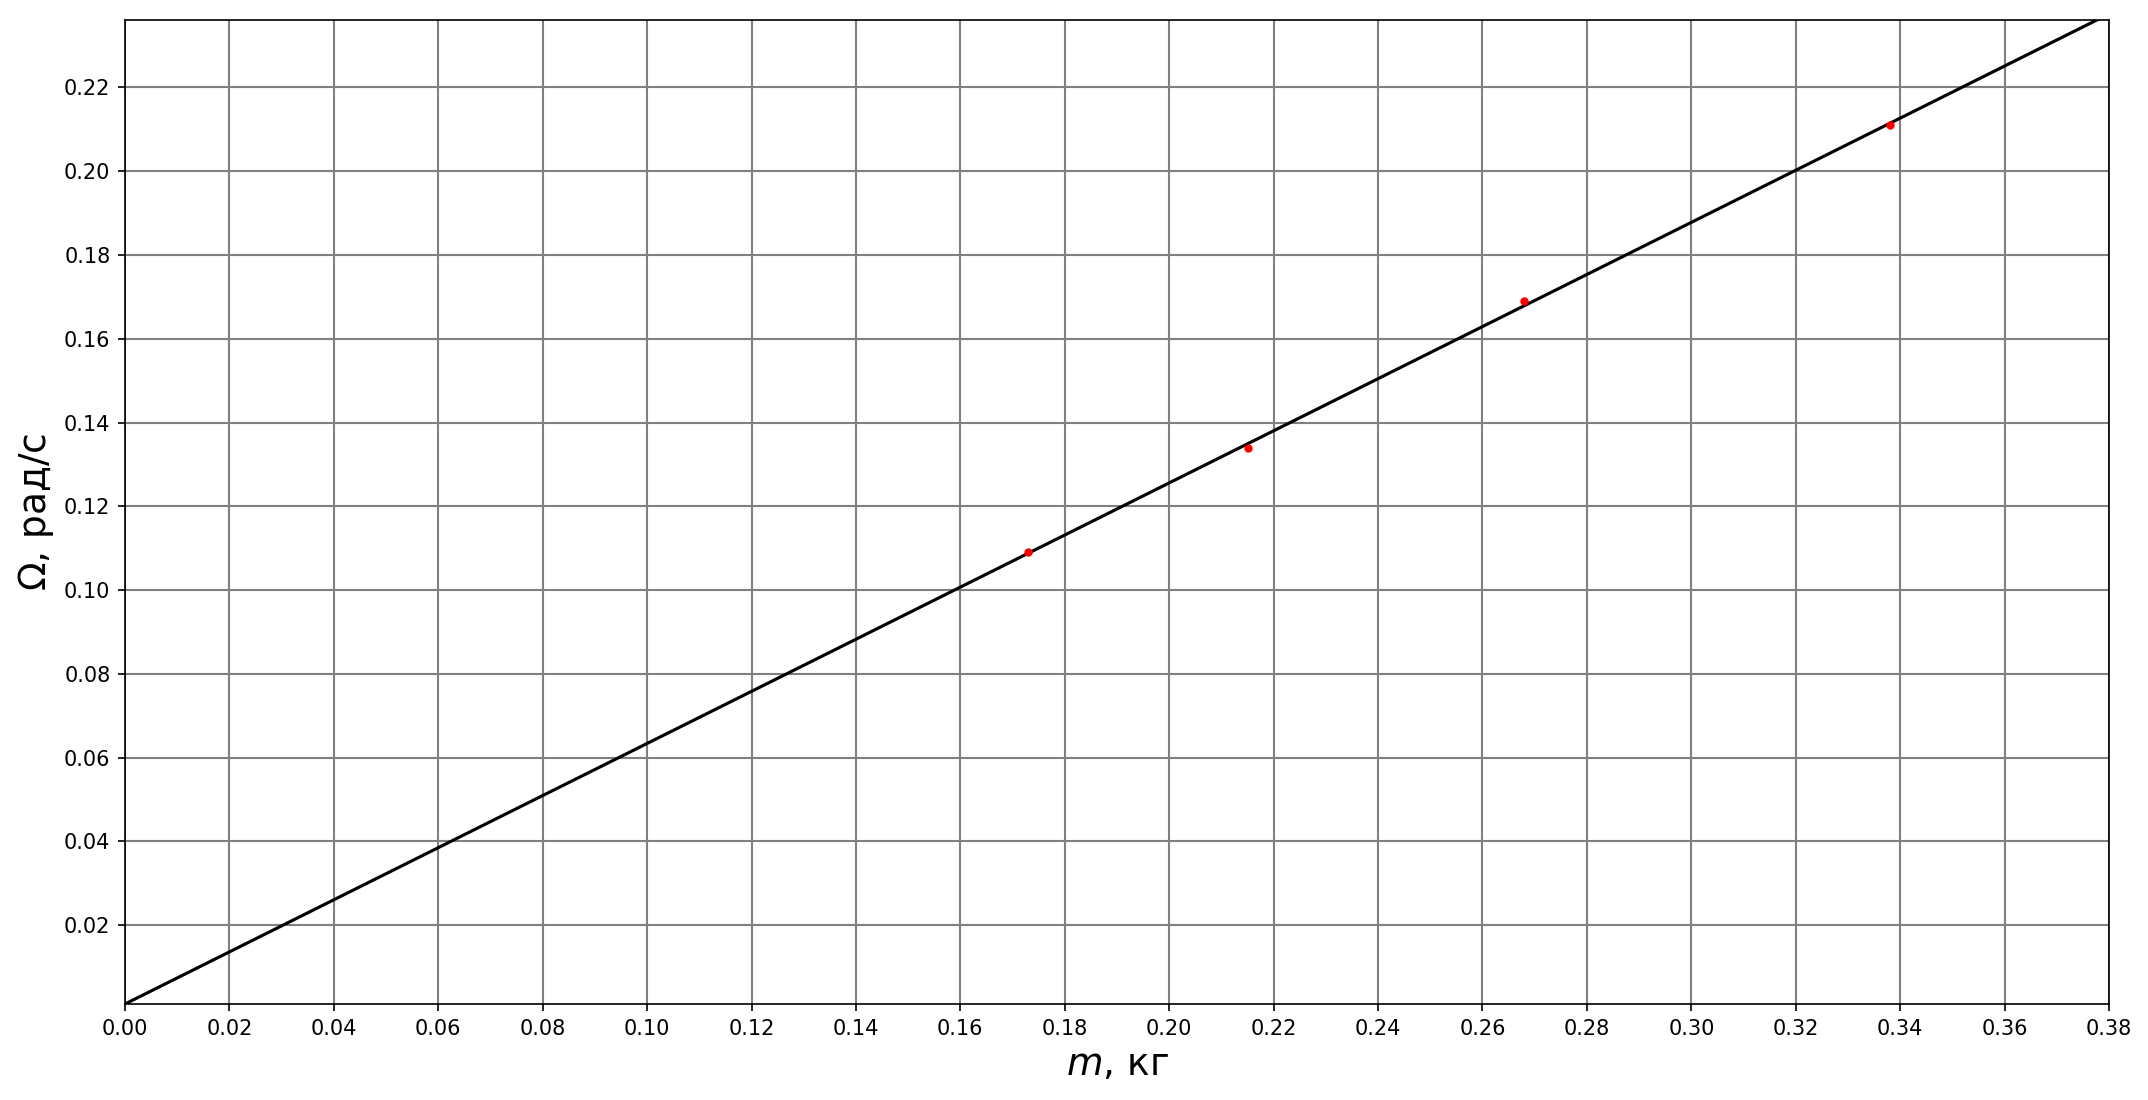
\includegraphics[scale = 0.5]{Screenshot 2023-11-15 141751.png}
    \caption{$\Omega(m)$}
    \label{fig:enter-label}
\end{figure}

Моменты сил трения при различных нагрузках представлены в таблице 3.
\[ M_{\text{тр}} = F_{\text{тр}}l = \Omega_{\text{тр}} I_z \omega_0\]
\[ \varepsilon_{M_{\text{тр}}} = \sqrt{\varepsilon_{\alpha}^2 + \varepsilon_{Iz}^2 + \varepsilon_{\omega_0}^2} = 20,19 \%\]

\begin{table}[!ht]
    \centering
    \begin{tabular}{|l|l|l|l|l|}
    \hline
        $m$, г & 338 & 268 & 215 & 173 \\ \hline
        $M_{\text{тр}}$, $\text{Н}\cdot\text{м}$ & 0,002 & 0,0021 & 0,002 & 0,0019 \\ \hline
    \end{tabular}
    \caption{моменты сил трения при различных нагрузках}
\end{table}

\section*{Вывод}

В работе была определена частота вращения ротора гироскопа с помощью измерения скорости прецессии гироскопа, полученое значение частоты $ \nu = (379,66 \pm 8,28) \text{ Гц } (\varepsilon_{\nu} = 2,18 \%)$. Также в ходе эксперимента частота была определена с помощью осциллографа, полученное значение 381,5 Гц. Полученные значения близки, можно считать эксперимент удачным, но при попытке расчитать момент силы трения, действующей на гироскоп из-за прецессии были получены не соответствующие реальности данные, скорее всего, момент силы трения изменялся в пределах большой погрешности (20\%), на которую сильно повлияла цена деления шкалы для определения изменения вертикального угла гироскопа, из-за чего полученные данные некорректны.

\end{document}

